\section{Caravaggio}\label{caravaggio}


\begin{figure}
\centering

\includegraphics{Screenshot_2023-10-03_204548.png}
\caption{Screenshot 2023-10-03 204548.png}
\end{figure}

Informazioni Generali

Età:

Data di nascita:

Luogo di nascita:

Razza:

Classe:

Alleati:

Nemesi:

Alias:

Professione:


\subsection{1. Descrizione Generale}\label{descrizione-generale}


\begin{figure}
\centering
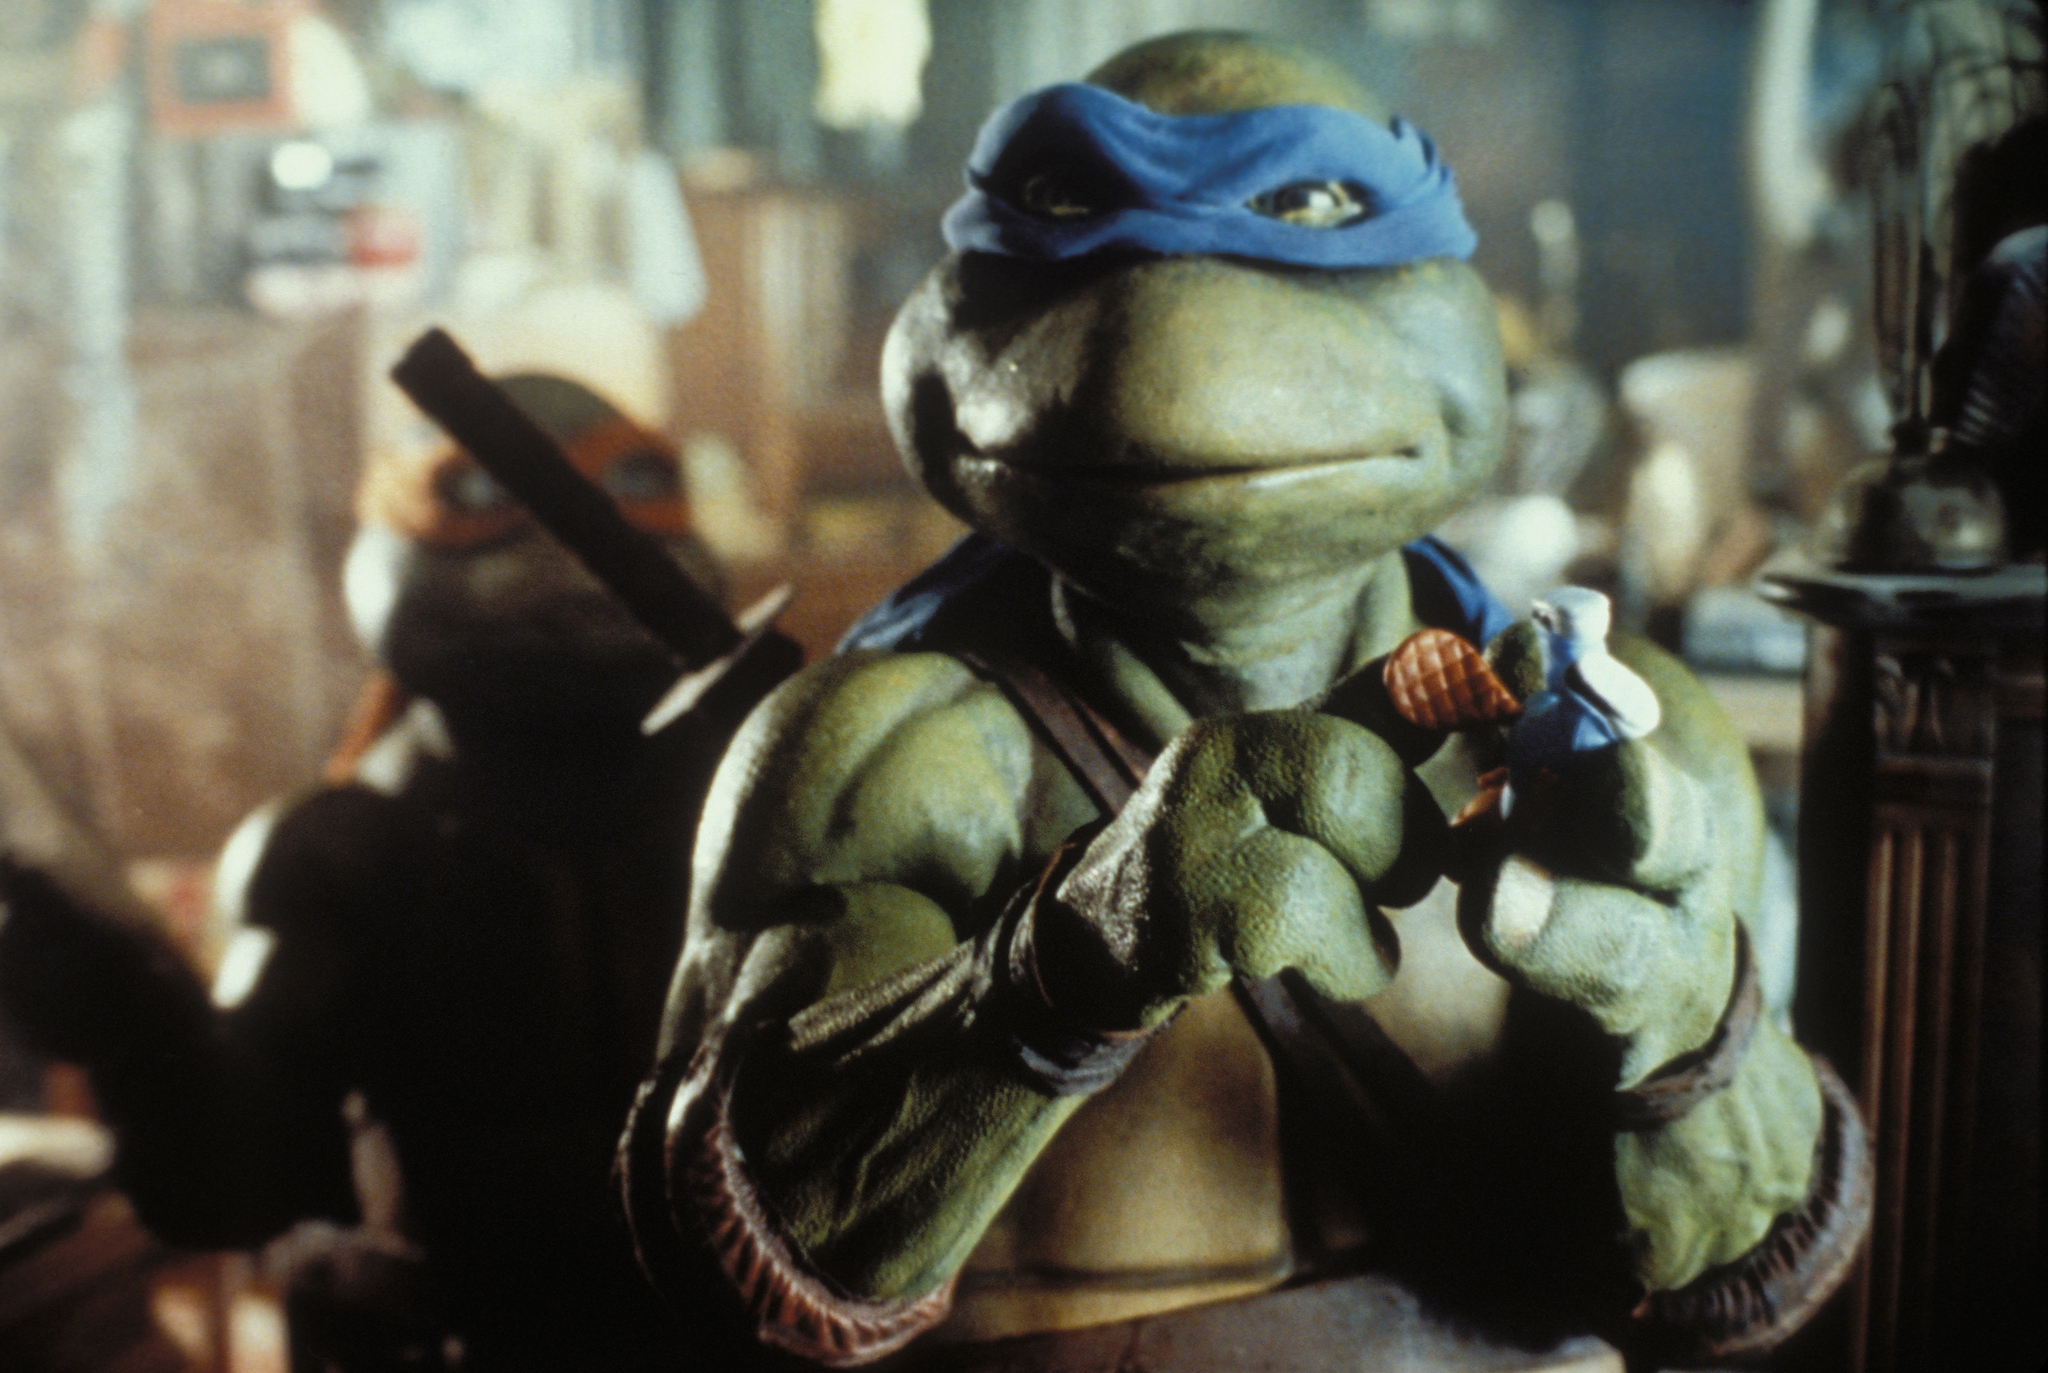
\includegraphics{foto_caravaggio.jpg}
\caption{foto caravaggio.jpg}
\end{figure}

Caravaggio è un monaco turtlefolk guerriero. La sua pelle verde scura e
il robusto guscio marrone lo distinguono tra gli altri della sua razza.
Caravaggio è noto per la sua lealtà, il suo coraggio e la sua
determinazione.

\begin{quote}
Citazione {[}location{]}
\end{quote}

\subsection{2. Biografia}\label{biografia}


Caravaggio è stato adottato da Splinter, un monaco mausefolk, insieme ai
suoi quattro fratelli. Splinter li ha cresciuti e addestrati alle arti
marziali, insegnando loro l'importanza della disciplina e della
protezione degli altri. Durante un viaggio in nave, un tremendo
naufragio ha separato Caravaggio dalla sua famiglia. Ha passato anni a
cercarla, senza mai darsi per vinto, ma non l'ha mai trovata.

\subsection{3. Carriera}\label{carriera}


Caravaggio ha trovato una nuova casa nelle terre di Valtara, dove ha
messo le sue abilità da combattente a servizio della gilda dei
Protettori. La sua esperienza in combattimento lo ha reso un membro
prezioso dell'organizzazione, impegnato a proteggere la regione dagli
